% !TeX root = ../paper.tex
% !TeX encoding = UTF-8
% !TeX spellcheck = en_US

\section{Self-Healing}\label{sec:self-healing}
  Self-healing is an integral part of self-adaptive systems and the focus of this paper.
  It combines properties of
  (i) fault-tolerant systems, which handle transient failures and mask permanent ones to ensure system availability,
  (ii) self-stabilizing systems, which are non-fault masking and converge to the legal state in a finite amount of time, and 
  (iii) survivable systems, which maintain essential services and recover non-essential ones after intrusions have been dealt with~\cite{PsaierSurvey}.
  A widely-used definition for self-healing systems is from \citeauthor{Ghosh}~\cite{Ghosh}:

  \begin{quote}
    The key focus [...] is that a self-healing system should recover from the abnormal (or \enquote{unhealthy}) state and return to the normative (\enquote{healthy}) state, and function as it was prior to disruption.
  \end{quote}

  This definition is very broad, but one can argue that the key aspect of self-healing systems are recovery oriented functionalities that bring the system back to the healthy state, which neither sole fault-tolerant systems nor sole survivable systems encompass~\cite{PsaierSurvey}.

  Like in an autonomous system, the main component in a self-healing system is the self-healing manager.
  It runs a control loop with three stages that is a reduced version of the autonomic control loop, also referred to as MAPE-K loop~\cite{ibm_autonomic}.
  The self-healing loop consists of the following three main stages~\cite{PsaierSurvey}:

  \begin{description}
    \item[Detect] The self-healing manager filters the status information about the running system and reports suspicious events and detected degradations.
    \item[Diagnose] The diagnosis stage performs root cause analysis on the received reports from the previous stage and calculates a recovery strategy.
    \item[Recover] In the recovery phase the manager applies the strategies to the system while he avoids any unpredictable side effects.
  \end{description}

  These three stages reflect the definition of self-healing.
  \Cref{fig:self-healing-loop} shows the mapping of those stages to the MAPE-K control loop.
  There are two different ways, how a software system can be equipped with the above mentioned self-healing capabilities:

  \begin{figure}
    \centering
    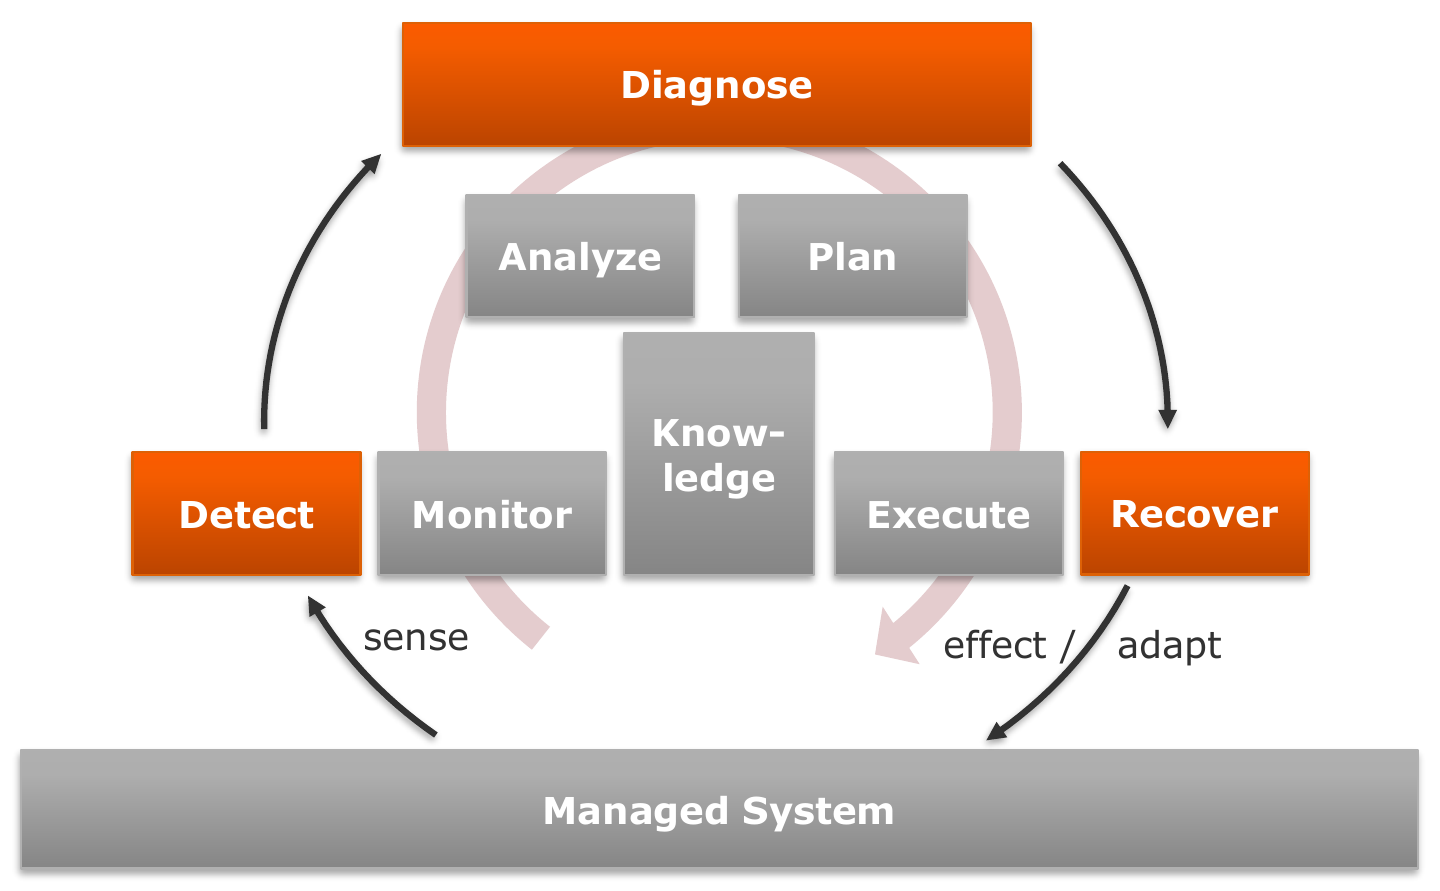
\includegraphics[width=.9\linewidth]{reduced-control-loop}
    \caption{Condensed autonomic control loop as the self-healing loop}
    \label{fig:self-healing-loop}
  \end{figure}

  The first approach is a software application with built-in self-healing logic.
  This means that the self-healing manager is within the application code and is able to access internal state and mechanisms.
  This can be an advantage as the application is a white box and the self-healing logic can use detailed status information and even domain knowledge for detection, analysis and recovery.
  At the other hand, this also means that the healing logic is tied to the application increasing coupling and violating the separation of concerns principle.
  If the application starves the self-healing manager may starve as well.

  The second approach is an external self-healing manager provided as an infrastructural component or as third-party service.
  The self-healing logic runs in isolation from the application code and can therefore treat the application only as a black box and has to use external metrics to judge the application's health.
  It's the current state of the art for monitoring, health management and scaling logic~\cite{ToffettiMicroservices}.
  The external management logic has to be itself resilient, fault-tolerant, and scalable for being able to heal the application.
  Using third party services or services provided by the infrastructure provider could lead to vendor lock-in.
  There are also open-source alternatives that include self-healing capabilities and can be used as middleware between cloud infrastructure and the application, such as \gls{kubernetes} or Mesosphere.

\subsection{Architecture-based self-healing}
  In the past most self-healing capabilities were included in the application code itself.
  This has the downside that the self-healing adaption engines and rules are tightly coupled to the application code and can't be reused.
  Researchers have therefore developed ways to generalize self-healing mechanisms.
  One approach are architecture-based self-healing systems, in which external self-healing managers perform repairs on the level of software components and connectors of the monitored systems~\cite{DashofyArchitecture}.
  The assumption of those approaches is that the component boundaries are the most loosely coupled points in the software system and can be reconfigured to allow changes in the architecture during runtime.

  \citeauthor{DashofyArchitecture} present the infrastructure to develop and run an architecture-based self-healing system that focuses on event-based software architectures in~\cite{DashofyArchitecture}.
  They chose event-based architectures, because all included components can only communicate via events and show a significant degree of autonomy.
  This reduces coupling of the components and makes changes from the outside to the system possible.

\subsection{Self-healing microservices}
  Microservice architectures take isolation of software components to the next level and improve the autonomy of the components (services).
  This makes applying repairs from the outside of the application easier, because services are decoupled, autonomous, and scalable and service boundaries are well-defined.
  External self-healing managers can monitor the microservices of the application and apply repairs to the failing or misbehaving ones by replacing the service with another one and rerouting the messages to the new instance.
  This is where the self-healing capabilities of the aforementioned cloud tools (refer to \cref{sec:introduction}) and \gls{kubernetes} can be used.

  In contrast to external self-healing managers, \citeauthor{ToffettiMicroservices} propose a self-healing system with the self-healing logic built into a microservice application.
  They leverage standard methods from distributed systems (\ie consensus algorithms) to assign self-management (includes self-healing) functionality to some nodes of the distributed application.
  The selected nodes form a hierarchy and perform different parts of the self-management logic.
  This means that the self-management logic is distributed in the cluster to overcome the connectedness to the application code~\cite{ToffettiMicroservices}.

\subsection{Self-healing in cloud environments}\label{sec:self-healing:cloud}
  As more and more applications are deployed in cloud environments, developers must consider the implications of running their software in the cloud.
  The Reactive Manifesto~\cite{reactivemanifesto} records the requirements, which today's software is facing.
  It asks for more resilient and responsive systems and postulates that resilience can be achieved by replication, containment, isolation, and delegation.
  Recovery should be handled by an external component to the application.
  This could be a self-healing manager.
  If the self-healing manager is run external to the application, it must itself be resilient to failures.

  Yesterday's software was deployed on bare metal or virtual machines, but in the cloud multiple layers of abstractions and virtualizations are used.
  Most of the time this is transparent to the application as \gls{paas} solutions are used.
  This means that compute units are much easier to scale, exchange and expand.
  On the other hand, self-healing strategies in cloud environments differ significantly from traditional ones, because the self-healing manager has no control over the underlying infrastructure and must work on higher abstraction levels.

  While systems and software components can fail in various ways and research has come up with general failure classifications and resolutions~\cite[Tab.~1]{PsaierSurvey} for any software systems, failures in cloud environments can be reduced to one failure class: a node or component is detected unreachable.
  Although an unreachable node can have different root causes on the infrastructure level, the impact on the system is the same.
  Because application developers have no control about the infrastructure in a cloud deployment, they have to find other ways besides repairing the infrastructure to heal from failures in the cloud.
  Node failures can be detected via heartbeat messages or latency metrics and a common recovery strategy is the redeployment of the software that was running on the node on another node.

  Research approaches that deal with these challenges for self-healing systems in the cloud are \citeauthor{StackCloud}~\cite{StackCloud}, who developed an hierarchical approach using a master-slave architecture to provide flexible and high available self-healing functionality in a cloud architecture, and \citeauthor{gru}~\cite{gru}, who have a similar approach to \gls{kubernetes}.
  They developed their own self-healing container orchestration tool, called Gru, that targets microservice architectures deployed in containers.

\section[Kubernetes]{\gls{kubernetes}}\label{sec:kubernetes}
  % https://kubernetes.io/docs/concepts/overview/what-is-kubernetes/
  \Gls{kubernetes} is an open-source platform for automating and managing distributed software in the cloud.
  It heavily relies on container technology and supports declarative configuration of the managed containers.
  \Gls{kubernetes} was developed by Google and is open-source software since 2014~\cite{kubernetes}.

  % https://kubernetes.io/docs/concepts/overview/components/
  \Gls{kubernetes} is build on top of existing \gls{paas} solutions and consists of a master-slave architecture, which is depicted in \cref{fig:kubernetes-architecture}, forming a cluster.
  Slave nodes, \gls{kubernetes} calls them only \enquote{nodes}, are responsible for executing and maintaining the actual application via an underlying container runtime.
  Most of the time Docker~\cite{docker} is used.
  The nodes also run \gls{kubernetes} components that manage cluster networking (\texttt{kube-proxy}) and interact with the container runtime and the master to monitor and manage the pods of the local node (\texttt{kubelet}).
  % https://kubernetes.io/docs/concepts/workloads/pods/pod-overview/
  Pods are the smallest deployment unit in \gls{kubernetes} and consist of the application container (or multiple), connected resources, such as storages or network addresses, and the configuration options.
  The container runtime, \texttt{kube-proxy} and \texttt{kubelet} form the \gls{kubernetes} runtime environment~\cite{kubernetes}.

  \begin{figure}
    \centering
    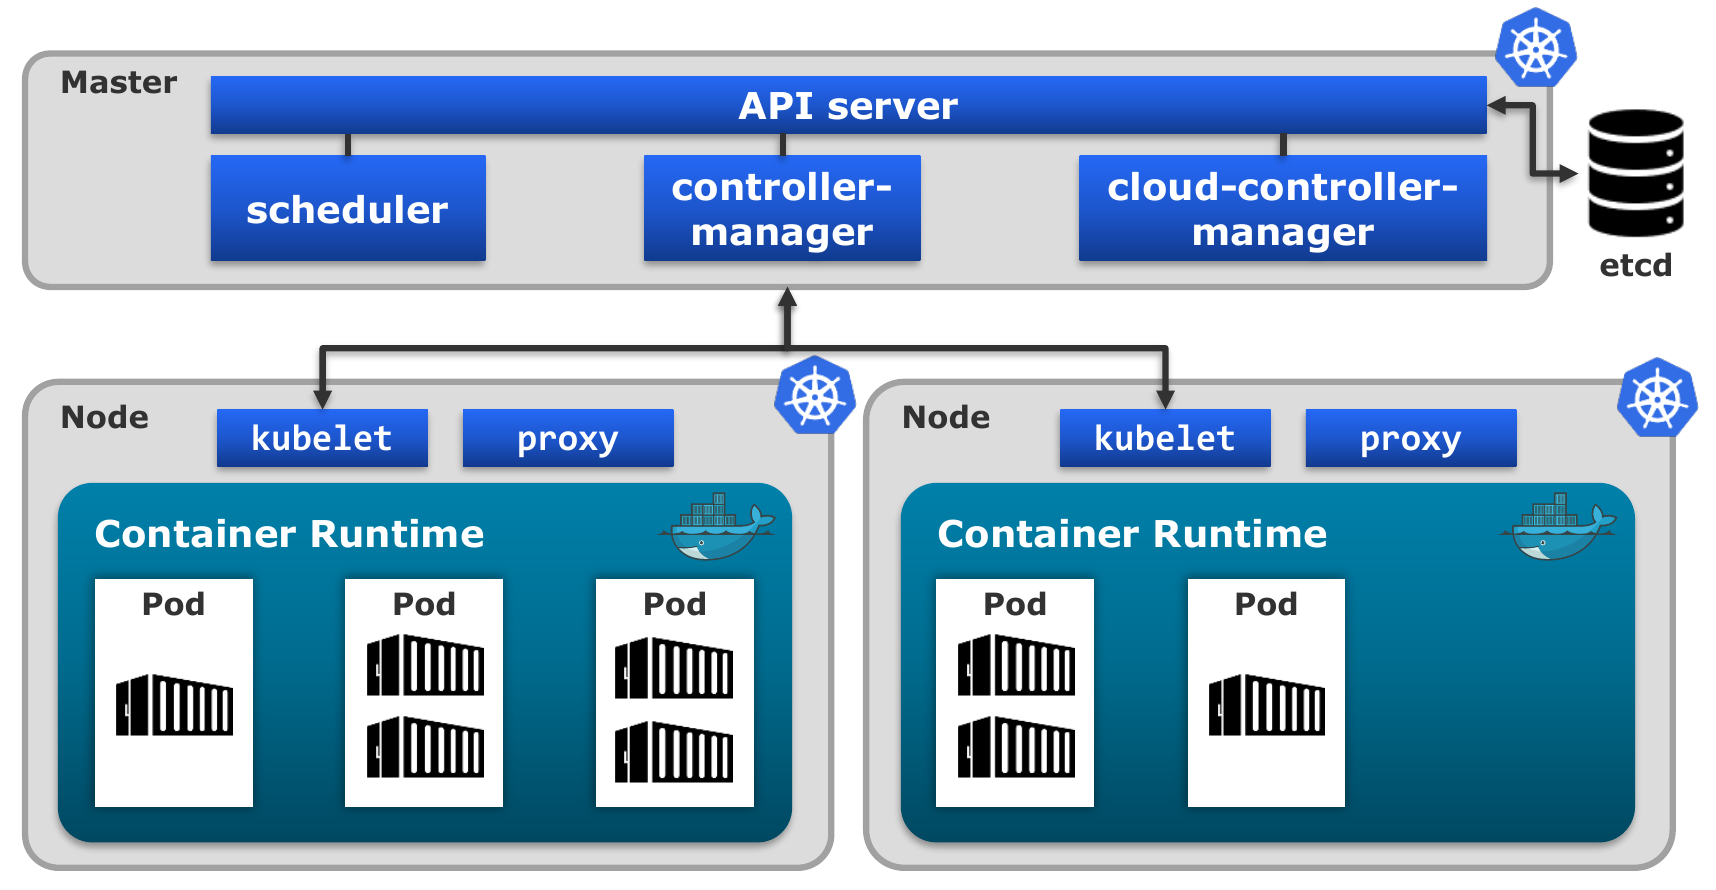
\includegraphics[width=.9\linewidth]{k8s-architecture}
    \caption{\Gls{kubernetes} architecture}
    \label{fig:kubernetes-architecture}
  \end{figure}

  The \gls{kubernetes} master components provide the cluster's control plane.
  As shown in the upper third of \cref{fig:kubernetes-architecture}, they typically run only on one node, which does not run application pods.
  However, the components can be executed on any node in the cluster.
  The master components include
  (i) the \texttt{kube-apiserver} that exposes the control options to the user and other software,
  (ii) an \texttt{etcd}~\cite{etcd} instance as store for all cluster data,
  (iii) the \texttt{kube-scheduler}, which schedules newly created pods to the nodes in the cluster,
  (iv) the \texttt{kube-controller-manager}, which runs Node and \glspl{pod controller}, and
  (v) the \texttt{cloud-controller-manager} to interact with the underlying cloud providers~\cite{kubernetes}.

  % https://kubernetes.io/docs/concepts/overview/working-with-objects/kubernetes-objects/
  For the declarative configuration and management of the application, \gls{kubernetes} employs the \gls{kubernetes} object model.
  All entities of the \gls{kubernetes} runtime are represented as description objects.
  The entirety of those objects represents the cluster state.
  Each object consists of three parts:
  (i) the object's metadata, such as name, version or labels,
  (ii) the object \texttt{spec}, which describes the desired state for the object and is provided by the user, and
  (iii) the object \texttt{status}, which describes the actual state of the object.
  Users of \gls{kubernetes} therefore only provide the object's metadata and \texttt{spec} to declare the desired deployment of their containerized applications on nodes and policies around how the application should behave.
  \Gls{kubernetes} will constantly update the \texttt{state} of the objects according to the observed cluster state and takes corrective actions in the cluster to ensure that the cluster state matches the desired one declared in the objects' \texttt{spec}~\cite{kubernetes}.

  % https://kubernetes.io/docs/concepts/overview/working-with-objects/labels/https://kubernetes.io/docs/concepts/overview/working-with-objects/labels/
  % should I describe labels as well?
